%-------------------------------------------------------------------------------
\section{Introduction}
%-------------------------------------------------------------------------------

Web applications today own, store, and sell user data, often without the user's knowledge or
explicit consent~\cite{nytimes:fb, npr:data}. This has dangerous consequences for both users and
application developers: data leaks~\cite{breach:twitter, breach:fb, breach:marriott, breach:quora}
has led to loss of livelihoods and lawsuits. Granting web applications such complete data
ownership clearly fails to protect users' privacy. 

However, a world in which the user has complete data ownership is equally problematic. Although
theoretically feasible~\cite{amber, w5, blockstack, bstore}, this model results in an arguably even
less desirable world for users. 
%
Applications that must compute on per-user, filesystem-esque storage become slow and limited, run
as JavaScript in users' browsers, and without the flexibility and easy of programming over SQL
databases with application-specific schemas.  Service-side computation and data sharing between
users---the main reason users use applications to begin with---becomes cumbersome, especially with
the addition of access control and authentication needed in order to access each users' data
individually. Furthermore, users are burdened with long-term data maintenance and storage: solutions
that use PKI, such as Blockstack~\cite{blockstack}, require users to maintain a master private key,
a cumbersome and fragile solution in which losing the key results in permanent loss of all the
user's data.
%
Finally, the current business model in which applications profit from user data, becomes infeasible,
requiring that users change the way they pay for services \lyt{this might not be a bad thing, though}.

This paper proposes a new model for web applications that balances users' desire for privacy with
their desire for application utility. In this model, users subscribe to applications by granting a
time-limited lease to their data, with the provision that the application may retain only
de-identified information once the user unsubscribes. Users flexibly switch between a
privacy-preserving unsubscribed mode and an identity-revealing subscribed mode at any time without
permanently losing their data. Applications can continue to operate using their current web
architecture, retaining their revenue model, performance and reliability, and utility for their
users. Applications do not need to access any removed unsubscribed users' data, simplifying the
storage of this data when users enter privacy-preserving mode.
Figure~\ref{fig:world} illustrates this flexible transfer of data ownership in our new model,
compared to the two extremes of complete user ownership and complete application ownership of user
data.

\begin{figure*}[ht!]
    \centering
    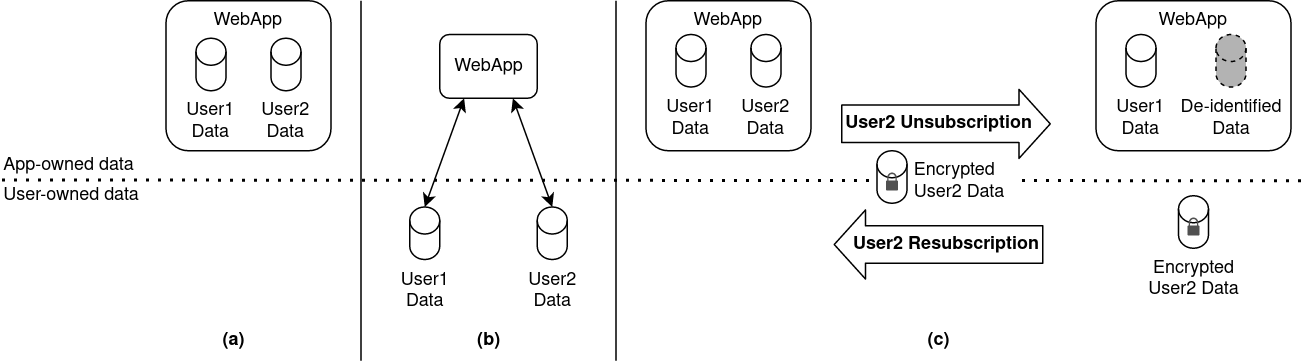
\includegraphics[width=\textwidth]{img/worlds}

    \caption{\textbf{(a)} The existing world of web applications, with applications maintaining and
    owning user data; \textbf{(b)} A world in which users have complete ownership of their data in cloud or local
    storage, and grant applications access to their data;
    \textbf{(c)} Our proposed model, which allows users to switch between privacy-preserving unsubscribed
    mode (right) and identity-revealing subscribed mode (left).}
    \label{fig:world}
\end{figure*}

This model clearly benefits the user: they can choose privacy at any time, without permanently
losing their accounts or affecting the utility of the applications for others.  But more
importantly, the model benefits application developers as well. Recent laws such as the European
Union's General Data Protection Regulation (GDPR)~\cite{eu:gdpr} and California's Consumer Privacy
Act (CCPA)~\cite{ca:privacy-act} codify users' rights to data ownership, granting users the right to
request erasure of information related to them, and creating incentives web applications to adopt
this model of flexible privacy. With this model, applications can support the (legally mandated)
right to be forgotten, while allowing its departing users to easily come back. Applications can
still use subscribed users' data to generate profit, and retain use of de-identified data even when
users unsubscribe; this ensures that the application holds only identifying data for currently subscribed users,
reducing the amount of compromising data in the system at any time.

Although applications increasingly support GDPR unsubscription requests, the current state of
unsubscription and resubscription is far from ideal. Unsubscription is often impossible or
cumbersome (users often contact the developers or customer support directly in order to
unsubscribe)~\cite{jdm}, and the implementation of unsubscription is manual, coarse-grained and
error-prone, and can fail to completely de-identify the user.  Even worse, no existing application
(to our knowledge) supports privacy-preserving unsubscription with the possiblity of resubscription.
Application unsubscription thus permanently deletes years or even decades of accumulated application
data, costing both users and the web application, and creating little incentive to lower barriers to
unsubscription. 

In order to make this model of flexible privacy and data ownership possible, we must solve the many
challenges faced by application developers. Key among these are the requirements for applications to
selectively retain unsubscribed users' data for legal purposes or application utility without also
identifying the user, and to allow the user to resubscribe at any time to their last-known
subscribed state. The complex data transformations required by user unsubscription and
resubscription highlight the need for new tools that allow developers to easily and systematically
automate the process.
%For example, 
%many applications require that some information remains
%post-unsubscription, for legal or necessary application use, but retained data can identify a user
%in complex ways: both user identifiers (\eg usernames) and structural \emph{correlations} between
%application data records (\eg between users and posts, or posts and tags) may reveal identifying
%information. Without a systematic way to anonymize user identifiers and \emph{decorrelate} these
%potentially identifying structural correlations, many developers have chosen to either entirely
%delete all sensitive data at the expense of other subscribed users, or leave identifying information
%unchanged at the expense of unsubscribed users.
%how application data and data correlations need to change when a user
%unsubscribes, and support automatic resubscription and recorrelation of users with their account
%data at any time.

In the rest of this paper, we describe in more detail the state of unsubscription and resubscription in
web applications today, and the challenges of implementing it correctly.  We then present \sys, a
system that provides abstractions and mechanisms to help developers of databased-backed web
applications achieve correct, privacy-compliant user unsubscription and resubscription without
onerous labor, and without adding undue overheads.
